\documentclass[conference, twocolumn]{IEEEtran}

\usepackage[utf8]{inputenc}
\usepackage[T1]{fontenc}
\usepackage{amsmath,amssymb}
\usepackage{graphicx}
\usepackage{booktabs}
\usepackage{hyperref}
\usepackage{cite}
\usepackage{multirow}
\usepackage{array}
\usepackage{float}
\usepackage{siunitx}
\usepackage{xcolor}
\usepackage{balance}

\graphicspath{{../figures/}}

\begin{document}

\title{A Comparative Study of Three Classical Machine Learning Algorithms for Multi-Class Network Intrusion Detection on the NSL-KDD Dataset}

\author{
\IEEEauthorblockN{Sudip Adhikari\textsuperscript{1}}
\IEEEauthorblockA{
\textsuperscript{1}Softwarica College of IT \& E-Commerce\\
(Coventry University)\\
Kathmandu, Nepal\\
}
}

\maketitle

\begin{abstract}
Network intrusion detection has become a moving target. Attacks change shape, and rule-based detection systems struggle to keep up. Machine learning offers a way to flag suspicious traffic by learning what attacks look like, but the choice of algorithm matters. This paper compares three classical machine learning algorithms --- Logistic Regression, Random Forest, and XGBoost --- on the NSL-KDD benchmark for five-class intrusion detection covering Normal, Denial-of-Service (DoS), Probe, Remote-to-Local (R2L), and User-to-Root (U2R) traffic. Each model is trained under identical conditions with one-hot encoded categorical features, standardised numerical features, and SMOTE applied per cross-validation fold to address severe class imbalance. Stratified 5-fold cross-validation is paired with held-out evaluation on the official KDDTest+ split. XGBoost achieves the highest test accuracy (78.66\%), the highest macro F1 (0.6337), and the strongest performance on rare attack classes, while Logistic Regression remains surprisingly competitive on weighted F1 thanks to strong majority-class performance. All three models show a substantial gap between cross-validation and held-out test scores --- a gap that the paper attributes to NSL-KDD's deliberate inclusion of unseen attack variants in the test set, and which we argue is more important to discuss than to hide. Feature importance analysis identifies a small set of network flow attributes (\texttt{service\_eco\_i}, \texttt{flag\_S0}, \texttt{dst\_host\_serror\_rate}) that carry most of the discriminative information.
\end{abstract}

\begin{IEEEkeywords}
Network Intrusion Detection, Machine Learning, NSL-KDD, Classification, Random Forest, XGBoost, Logistic Regression, Class Imbalance, SMOTE
\end{IEEEkeywords}

%% ============================================================
\section{Introduction}
%% ============================================================

The number of organisations that depend on networked services keeps rising, and so does the number of people who try to break into them. Intrusion detection systems (IDS) sit between the network and the host and try to flag traffic that looks like an attack. Traditional IDS implementations rely on signature matching: every connection is compared against a database of known attack patterns~\cite{kdd99}. This works well for attacks that have already been catalogued but offers little protection against new attacks or attacks that have been slightly modified to evade detection.

Machine learning offers a different angle. Rather than coding rules by hand, an ML-based detector learns the difference between normal and malicious traffic from labelled examples. Once trained, the same model can sometimes flag previously unseen attacks if they share characteristics with attacks the model has already learned about. Two decades of research --- including a long line of studies built on the KDD Cup 1999 and NSL-KDD benchmarks~\cite{tavallaee2009} --- have established this approach as a serious complement to signature-based detection.

There are, however, two things that the published literature on NSL-KDD often gets wrong. The first is that many studies report results from only one or two algorithms, which makes it impossible to tell whether their winning model is genuinely strong or simply the better of two weak choices. The second is that many studies report only overall accuracy. On NSL-KDD, where the Normal class accounts for roughly half of all training records, a classifier that labels every connection as Normal would still score around 53\% accuracy --- a useless detector with respectable-looking metrics.

This paper takes a different approach. We compare three algorithms that represent three different paradigms (linear, bagging-ensemble, boosting-ensemble), train them under identical conditions, and evaluate them with per-class metrics. The contributions are as follows:

\begin{enumerate}
    \item A controlled comparison of Logistic Regression, Random Forest, and XGBoost on the full five-class NSL-KDD problem, using identical preprocessing, identical class-imbalance handling, and identical evaluation.
    \item Per-class precision, recall, and F1 reporting in addition to overall metrics, with explicit discussion of how the rare R2L and U2R classes behave.
    \item An honest treatment of the gap between cross-validation and held-out test performance --- a gap many papers underemphasise --- and a discussion of what causes it.
    \item Feature importance analysis identifying the small set of network attributes that drive most predictions, which we argue offers practical value for analysts deciding what to monitor.
\end{enumerate}

Section~II surveys prior work. Section~III describes the dataset. Section~IV details the methodology. Section~V presents and discusses results. Section~VI concludes with limitations and future work.

%% ============================================================
\section{Literature Review}
%% ============================================================

The KDD Cup 1999 dataset~\cite{kdd99} was the first widely used benchmark for evaluating intrusion detection systems. It was generated from the DARPA 1998 network traffic simulation and contained roughly 4.9 million connection records. Tavallaee et al.~\cite{tavallaee2009} later identified several problems with KDD Cup 1999, the most damaging of which was the presence of large numbers of duplicate records. Duplicates biased classifiers toward frequently occurring attack patterns and inflated reported accuracies. They responded with NSL-KDD, a refined version that removes the duplicates and adds a difficulty score per record. NSL-KDD has remained the most widely used benchmark for classical-ML intrusion detection research ever since.

Several studies have used NSL-KDD to compare classical algorithms. Ahmad et al.~\cite{ahmad2021} surveyed machine learning and deep learning approaches and reported that ensemble methods --- Random Forest in particular --- typically outperform single models. Their study, however, was largely binary (attack versus normal) rather than the full five-class formulation, and so it sidesteps the question of how the rare R2L and U2R families are handled.

Dhanabal and Shantharajah~\cite{dhanabal2015} ran J48 (a Decision Tree variant), Naive Bayes, and SVM on NSL-KDD. J48 achieved the best overall accuracy (around 81\%), but the authors note that Naive Bayes performed especially poorly on R2L and U2R, attributing this to the small number of training samples in those classes. This pattern --- strong overall accuracy but collapse on rare classes --- recurs throughout the NSL-KDD literature and motivates the per-class focus of the present study.

Ingre and Yadav~\cite{ingre2015} applied artificial neural networks to NSL-KDD and reported small improvements over classical methods at the cost of significantly higher training time and reduced interpretability. Gu and Lu~\cite{gu2021} proposed an XGBoost-based pipeline with feature selection and showed that careful feature reduction can both speed up training and slightly improve accuracy. Their work motivates the feature-importance analysis we report later.

The recurring observation that R2L and U2R remain hard regardless of algorithm has led to a separate line of work on imbalance handling. Panigrahi and Borah~\cite{panigrahi2018}, working on the related CICIDS2017 dataset, showed that SMOTE~\cite{chawla2002} improves minority-class detection at the cost of slightly increased false positives on majority classes. Recent comparative work~\cite{nature2026, applied2025} continues to call for systematic, like-for-like comparisons across algorithms with proper per-class reporting --- precisely the gap this paper sets out to address for the three-algorithm case.

%% ============================================================
\section{Dataset Description}
%% ============================================================

NSL-KDD~\cite{tavallaee2009} ships in two predefined splits: KDDTrain+ (125{,}973 records) and KDDTest+ (22{,}544 records). Each record represents a single network connection described by 41 features and a class label. The features fall into four families:

\begin{itemize}
    \item \textbf{Basic features (1--9)}: derived directly from the TCP/IP connection --- duration, protocol type (TCP, UDP, ICMP), service (HTTP, FTP, SMTP, etc.), source and destination byte counts, and connection flags.
    \item \textbf{Content features (10--22)}: payload-related signals including failed login attempts, root shell access, and file creation activity.
    \item \textbf{Time-based traffic features (23--31)}: statistics computed over a two-second time window, such as the number of connections to the same host and the percentage of connections with SYN errors.
    \item \textbf{Host-based traffic features (32--41)}: statistics computed over the past 100 connections to the same host.
\end{itemize}

Three of the 41 features are categorical (\texttt{protocol\_type}, \texttt{service}, \texttt{flag}); the remaining 38 are numerical. The 22 specific attack labels in NSL-KDD are conventionally collapsed into four high-level attack families plus Normal, following the original mapping from Tavallaee et al.

The class distribution is shown in Table~\ref{tab:classes} and visualised in Fig.~\ref{fig:class-dist}. The imbalance is severe and asymmetric. DoS and Normal together account for roughly 90\% of training records. R2L is rare in training (0.79\%) but jumps to 12.81\% in the test set --- this is not an error but a deliberate design choice in NSL-KDD: the test set deliberately contains attack subtypes that are absent or under-represented in training, which is what makes the dataset realistic and difficult.

\begin{table}[!ht]
\centering
\caption{NSL-KDD class distribution.}
\label{tab:classes}
\begin{tabular}{lrrrr}
\toprule
Class & Train & \% & Test & \% \\
\midrule
Normal & 67{,}343 & 53.46 & 9{,}711 & 43.08 \\
DoS    & 45{,}927 & 36.46 & 7{,}458 & 33.08 \\
Probe  & 11{,}656 &  9.25 & 2{,}421 & 10.74 \\
R2L    &      995 &  0.79 & 2{,}887 & 12.81 \\
U2R    &       52 &  0.04 &      67 &  0.30 \\
\midrule
\textbf{Total} & \textbf{125{,}973} & \textbf{100} & \textbf{22{,}544} & \textbf{100} \\
\bottomrule
\end{tabular}
\end{table}

\begin{figure}[!ht]
\centering
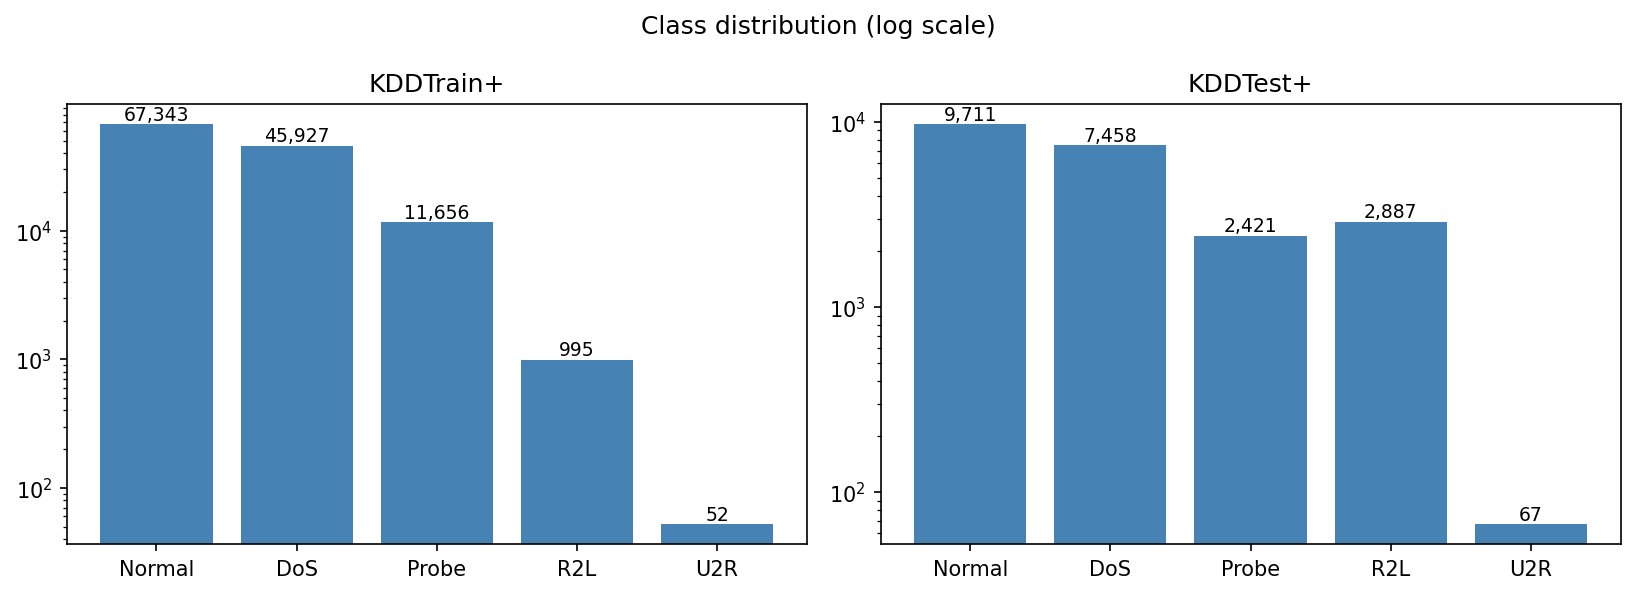
\includegraphics[width=\columnwidth]{class_distribution.png}
\caption{Class distribution on a log scale. Note the three orders of magnitude separating Normal/DoS from U2R.}
\label{fig:class-dist}
\end{figure}

%% ============================================================
\section{Methodology}
%% ============================================================

\subsection{Preprocessing}

The three categorical features (\texttt{protocol\_type} with 3 values, \texttt{service} with roughly 70 values, and \texttt{flag} with 11 values) are one-hot encoded. Encoding is applied to the union of train and test categories so that any service strings that appear only in the test set --- of which NSL-KDD has several --- are still represented. After encoding, the feature dimensionality grows from 41 to 122.

Numerical features are then standardised (zero mean, unit variance) using a scaler fit only on the training data. Standardisation is important for Logistic Regression because its coefficients otherwise depend on feature scales; tree-based methods do not require it but suffer no harm from it.

\subsection{Handling Class Imbalance}

The Synthetic Minority Over-sampling Technique (SMOTE)~\cite{chawla2002} is applied to address class imbalance. SMOTE interpolates between minority-class samples and their nearest neighbours to create new synthetic minority instances rather than copying existing ones, which would risk overfitting to specific samples.

A subtle but important detail is \emph{when} to apply SMOTE. We apply it inside each cross-validation fold, on the training side only, never on the validation side. Resampling the entire training set before splitting would leak synthetic samples derived from validation neighbours back into the training set and inflate cross-validation scores artificially. After cross-validation we resample the full training set once more for the final model fit; the held-out KDDTest+ set is never touched by SMOTE.

\subsection{Algorithms}

\textbf{Logistic Regression (LR)} is a linear, probabilistic classifier. We use the multinomial formulation with the L-BFGS solver and a maximum of 1{,}000 iterations. LR provides a baseline against which non-linear models can be compared.

\textbf{Random Forest (RF)}~\cite{breiman2001} is a bagging ensemble of decision trees trained on bootstrap samples with random feature subsetting at each split. We use 100 trees with no maximum depth and class-balanced weighting at the leaf level.

\textbf{XGBoost}~\cite{chen2016} is a gradient-boosting ensemble that fits trees sequentially, where each tree is trained to correct the residual errors of the trees that came before it. We use 200 trees of maximum depth 6, a learning rate of 0.1, and the histogram-based tree construction algorithm for speed.

We have intentionally kept hyperparameters conservative. Heavy tuning would obscure the comparison because each algorithm has a different sensitivity to its hyperparameter space, and aggressive tuning of one model would not reflect a fair comparison.

\subsection{Evaluation}

Models are evaluated using stratified 5-fold cross-validation on the training set, followed by a final evaluation on the held-out KDDTest+ set. We report the following metrics, both per-class and as weighted/macro averages:

\begin{equation}
    \text{Precision} = \frac{TP}{TP + FP} \quad
    \text{Recall} = \frac{TP}{TP + FN}
\end{equation}
\begin{equation}
    \text{F1} = 2 \cdot \frac{\text{Precision} \cdot \text{Recall}}{\text{Precision} + \text{Recall}}
\end{equation}

We additionally report ROC-AUC computed with the one-versus-rest strategy. Macro F1 averages the per-class F1 scores equally and is the most informative single number on imbalanced data because it punishes models that ignore rare classes; weighted F1 weights each class by support and rewards majority-class accuracy.

%% ============================================================
\section{Results and Discussion}
%% ============================================================

\subsection{Overall Performance}

Table~\ref{tab:overall} summarises the held-out test results. XGBoost leads on accuracy, macro F1, and ROC-AUC. Random Forest is fastest to train. Logistic Regression edges out the other two on weighted F1, but as the per-class breakdown will show, this is largely an artefact of strong majority-class performance.

\begin{table}[!ht]
\centering
\caption{Overall performance on KDDTest+. CV F1 is the mean weighted F1 across 5 folds on the training set.}
\label{tab:overall}
\begin{tabular}{lcccc}
\toprule
Algorithm & Acc.\,(\%) & Wt.\,F1 & Macro\,F1 & AUC \\
\midrule
LR      & 77.91 & 0.7631 & 0.5745 & 0.8970 \\
RF      & 75.05 & 0.7112 & 0.5382 & 0.9476 \\
XGBoost & \textbf{78.66} & 0.7582 & \textbf{0.6337} & \textbf{0.9537} \\
\bottomrule
\end{tabular}
\end{table}

The most striking observation does not appear in Table~\ref{tab:overall} directly. The cross-validation weighted F1 scores were 0.9756 (LR), 0.9987 (RF), and 0.9991 (XGBoost) --- effectively perfect. The held-out test scores fall by roughly 22 percentage points. This gap is not overfitting in the usual sense; it is a property of the dataset. KDDTest+ contains attack subtypes that do not appear in KDDTrain+, so the cross-validation score reflects performance on the training distribution while the test score reflects performance on a different distribution. Studies that omit the held-out evaluation often quote the cross-validation scores and create the impression of solved problem. They are reporting the wrong number.

\subsection{Per-Class Performance}

Table~\ref{tab:perclass} reports per-class F1 on KDDTest+. The pattern is consistent across all three models: Normal and DoS are easy, Probe is moderate, R2L is hard, U2R is hardest.

\begin{table*}[!ht]
\centering
\caption{Per-class F1-scores on KDDTest+.}
\label{tab:perclass}
\begin{tabular}{lccccc}
\toprule
Algorithm & Normal & DoS & Probe & R2L & U2R \\
\midrule
LR      & 0.8058 & 0.9028 & 0.7344 & 0.2976 & 0.1320 \\
RF      & 0.7800 & 0.8447 & 0.7614 & 0.1048 & 0.2000 \\
XGBoost & \textbf{0.8095} & 0.8788 & \textbf{0.7848} & 0.2597 & \textbf{0.4356} \\
\bottomrule
\end{tabular}
\end{table*}

XGBoost is the only model that obtains a usable F1 on U2R (0.4356, versus 0.20 and 0.13). On R2L, however, all three models struggle: even XGBoost only recalls 15\% of R2L attacks on the test set. Logistic Regression actually achieves the best R2L F1 (0.2976), which is at first surprising but consistent with the literature: linear models with class-balanced training tend to produce more diffuse decision boundaries that occasionally help on noisy minority classes.

\begin{figure}[!ht]
\centering
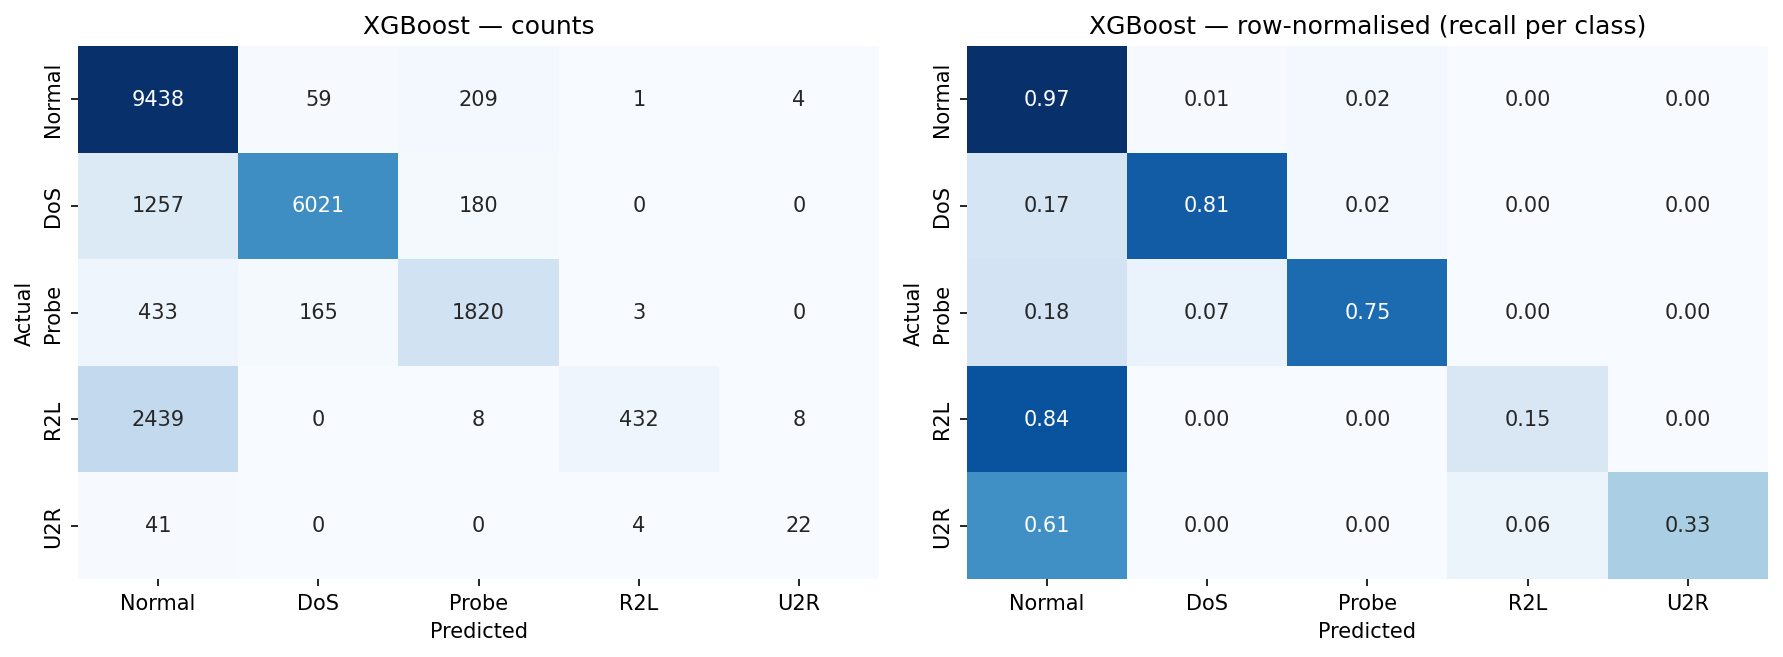
\includegraphics[width=\columnwidth]{cm_xgboost.png}
\caption{XGBoost confusion matrix on KDDTest+, with raw counts (left) and row-normalised (right) so the diagonal is per-class recall.}
\label{fig:cm-xgb}
\end{figure}

The XGBoost confusion matrix in Fig.~\ref{fig:cm-xgb} shows where the failures land. 84\% of R2L test attacks are misclassified as Normal, and 61\% of U2R attacks are also misclassified as Normal. The security implication is sobering: these are the most dangerous attacks in the dataset (unauthorised remote access and privilege escalation), and the model is most confident in calling them benign. Anyone deploying a classical-ML detector against R2L-class threats should expect a high false-negative rate and plan compensating controls accordingly.

\subsection{Feature Importance}

\begin{figure}[!ht]
\centering
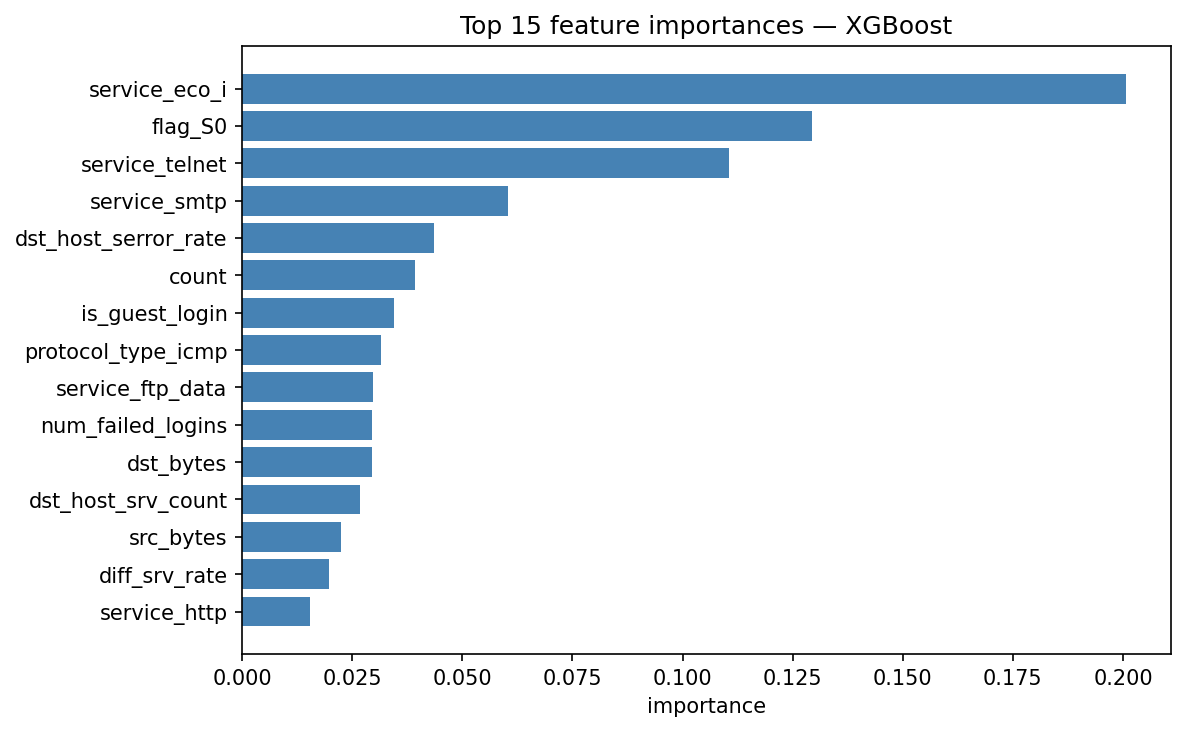
\includegraphics[width=\columnwidth]{fi_xgboost.png}
\caption{Top 15 feature importances from XGBoost.}
\label{fig:fi-xgb}
\end{figure}

Fig.~\ref{fig:fi-xgb} shows the top 15 features ranked by XGBoost importance. The top three (\texttt{service\_eco\_i}, \texttt{flag\_S0}, \texttt{service\_telnet}) account for roughly 40\% of the model's split decisions. \texttt{service\_eco\_i} indicates ICMP echo traffic, which appears heavily in probe attacks; \texttt{flag\_S0} marks connections where a SYN was sent but no SYN-ACK was returned, a textbook signature of SYN-flood and port-scan behaviour; \texttt{service\_telnet} flags Telnet traffic, which is rare in legitimate modern environments but heavily present in R2L brute-force attempts. These are quantities that a network administrator would already monitor; the value of the ML model is that it weighs them quantitatively and combines them with thirty-eight other signals.

\subsection{Discussion}

A few patterns deserve emphasis.

First, the difference between cross-validation scores and held-out test scores is the single largest effect in the experiment, larger than the differences between models. Studies that report only cross-validation results are not measuring what they appear to be measuring.

Second, the choice of metric matters enormously when the dataset is imbalanced. Weighted F1 and accuracy both place XGBoost and LR within roughly one percentage point of each other; macro F1 separates them by six points. On real intrusion detection deployments, where missing a single U2R attack is much worse than misclassifying ten Normal connections, macro F1 is the metric to optimise.

Third, ensemble methods are not uniformly better. Random Forest is faster to train than XGBoost but loses on every test-set metric except precision. The sequential boosting in XGBoost meaningfully helps on the rare classes, suggesting that the residual-fitting nature of boosting genuinely lets later trees specialise in the minority cases that earlier trees miss.

Fourth, even the best model in this study would be insufficient as a standalone production detector for R2L-class threats. The 15\% recall on R2L means that 85\% of these attacks would slip through. This is a known limitation of NSL-KDD and of classical approaches in general; production systems would need to layer additional detection (anomaly-based, payload-inspection, behavioural) to compensate.

%% ============================================================
\section{Conclusions}
%% ============================================================

We compared three classical machine learning algorithms --- Logistic Regression, Random Forest, and XGBoost --- on the full five-class NSL-KDD intrusion detection problem under identical preprocessing and evaluation conditions. XGBoost achieved the best test accuracy (78.66\%), the best macro F1 (0.6337), and the best detection of rare attack types, with R2L and U2R remaining hard for all three models. We also documented a roughly 22-percentage-point gap between cross-validation and held-out test scores, which we trace to the deliberate inclusion of unseen attack variants in NSL-KDD's test split.

The work has clear limitations. We used a single benchmark dataset, restricted to classical algorithms, and applied only one resampling strategy. Most importantly, NSL-KDD's underlying traffic is from 1998; modern attack patterns (HTTP-based exploits, modern DDoS, encrypted-channel exfiltration) are not represented. The strongest validation of an NSL-KDD-trained detector would be to apply it to a more recent benchmark such as CICIDS2017~\cite{panigrahi2018} and observe how well the model generalises. We leave this validation as future work along with cost-sensitive learning that explicitly penalises missed rare-attack detections more than false alarms on Normal traffic.

%% ============================================================

\section*{Acknowledgements}
The author thanks Softwarica College of IT \& E-Commerce and Coventry University for the academic environment in which this work was carried out, and the maintainers of the NSL-KDD dataset for providing a benchmark that has supported two decades of intrusion detection research.

%% ============================================================

\begin{thebibliography}{99}

\bibitem{kdd99}
KDD Cup 1999 Data. UCI Machine Learning Repository. Available: \url{http://kdd.ics.uci.edu/databases/kddcup99/kddcup99.html}

\bibitem{tavallaee2009}
M. Tavallaee, E. Bagheri, W. Lu, and A. A. Ghorbani, ``A detailed analysis of the KDD CUP 99 data set,'' in \textit{Proc. IEEE Symposium on Computational Intelligence for Security and Defense Applications (CISDA)}, pp. 1--6, 2009.

\bibitem{ahmad2021}
Z. Ahmad, A. S. Khan, C. W. Shiang, J. Abdullah, and F. Ahmad, ``Network intrusion detection system: A systematic study of machine learning and deep learning approaches,'' \textit{Transactions on Emerging Telecommunications Technologies}, vol. 32, no. 1, e4150, 2021.

\bibitem{dhanabal2015}
L. Dhanabal and S. P. Shantharajah, ``A study on NSL-KDD dataset for intrusion detection system based on classification algorithms,'' \textit{International Journal of Advanced Research in Computer and Communication Engineering}, vol. 4, no. 6, pp. 446--452, 2015.

\bibitem{ingre2015}
B. Ingre and A. Yadav, ``Performance analysis of NSL-KDD dataset using ANN,'' in \textit{Proc. International Conference on Signal Processing and Communication Engineering Systems (SPACES)}, pp. 92--96, 2015.

\bibitem{gu2021}
J. Gu and S. Lu, ``An effective intrusion detection approach using SVM with na\"ive Bayes feature embedding,'' \textit{Computers \& Security}, vol. 103, p. 102158, 2021.

\bibitem{panigrahi2018}
R. Panigrahi and S. Borah, ``A detailed analysis of CICIDS2017 dataset for designing intrusion detection systems,'' \textit{International Journal of Engineering \& Technology}, vol. 7, no. 3.24, pp. 479--482, 2018.

\bibitem{chawla2002}
N. V. Chawla, K. W. Bowyer, L. O. Hall, and W. P. Kegelmeyer, ``SMOTE: Synthetic Minority Over-sampling Technique,'' \textit{Journal of Artificial Intelligence Research}, vol. 16, pp. 321--357, 2002.

\bibitem{breiman2001}
L. Breiman, ``Random forests,'' \textit{Machine Learning}, vol. 45, no. 1, pp. 5--32, 2001.

\bibitem{chen2016}
T. Chen and C. Guestrin, ``XGBoost: A scalable tree boosting system,'' in \textit{Proc. 22nd ACM SIGKDD International Conference on Knowledge Discovery and Data Mining}, pp. 785--794, 2016.

\bibitem{nature2026}
``Anomaly-based intrusion detection on benchmark datasets for network security: a comprehensive evaluation,'' \textit{Scientific Reports}, vol. 16, 2026.

\bibitem{applied2025}
``Advanced IDS: a comparative study of datasets and machine learning algorithms for network flow-based intrusion detection systems,'' \textit{Applied Intelligence}, 2025.

\end{thebibliography}

\end{document}
